\documentclass{beamer}
\usepackage{fancyvrb}
\usepackage{animate}
\usepackage{multimedia}
\usepackage{hyperref}
\usepackage{amsmath}
\usepackage[latin1]{inputenc}
\usetheme{PaloAlto}
\usepackage[scaled=0.55]{helvet}

\title{Adaptive hp-DG Method with dynamically changing meshes for compressible Euler equations}
\author{\underline{Lukas Korous}, hp-FEM group}
\institute[Pilsen]{University of West Bohemia, Pilsen}

\begin{document}


% Feistauer
\def \SS{\mbox{\boldmath $S$}}
\def \va {\mbox{\boldmath $\varphi$}}
\def \nn {\mbox{\boldmath $n$}}
\def \vv {\mbox{\boldmath $v$}}
\def \uu {\mbox{\boldmath $u$}}
\def \w {\mbox{\boldmath $w$}}
\def \ww {\mbox{\boldmath $w$}}
\def \x {\mbox{\boldmath $x$}}
\def \f {\mbox{\boldmath $f$}}
\def \ff {\mbox{\boldmath $f$}}
%\def \g {\mbox{\boldmath $g$}}
\def \c {\mbox{\boldmath $c$}}
\def \dd {\mbox{\boldmath $d$}}
\def\DDD{\mbox{\boldmath$D$}}

\newcommand{\lo}{\left(}
\newcommand{\ro}{\right)} 
\newcommand{\bs}[1]{\textit{\textbf{#1}}}
\newcommand{\bsm}[1]{\boldsymbol{#1}}
\newcommand{\pds}[2]{\frac{\partial{#1}}{\partial{#2}}}
\newcommand{\pdv}[2]{\frac{\partial{#1}}{\partial{\bs{#2}}}}
\renewcommand{\d}[2]{\frac{d{#1}}{d{#2}}}
\newcommand{\mc}[1]{\mathcal{#1}}
\newcommand{\phib}{\bsm{\varphi}}
\newcommand{\esssup}{\operatornamewithlimits{ess\,sup}}


\def\be{\begin{equation}}
\def\ee{\end{equation}}
\def\bfig{\begin{figure}}
\def\efig{\end{figure}}
\def\bd{\begin{displaymath}}
\def\ed{\end{displaymath}}
\def\ba{\begin{array}}
\def\ea{\end{array}}

\newcommand{\bfa}{\mbox{\boldmath $a$}}
\newcommand{\bfb}{\mbox{\boldmath $b$}}
\newcommand{\bfc}{\mbox{\boldmath $c$}}
\newcommand{\bfd}{\mbox{\boldmath $d$}}
\newcommand{\bfe}{\mbox{\boldmath $e$}}
\newcommand{\bff}{\mbox{\boldmath $f$}}
\newcommand{\bfg}{\mbox{\boldmath $g$}}
\newcommand{\bfh}{\mbox{\boldmath $h$}}
\newcommand{\bfi}{\mbox{\boldmath $i$}}
\newcommand{\bfj}{\mbox{\boldmath $j$}}
\newcommand{\bfk}{\mbox{\boldmath $k$}}
\newcommand{\bfl}{\mbox{\boldmath $l$}}
\newcommand{\bfm}{\mbox{\boldmath $m$}}
\newcommand{\bfn}{\mbox{\boldmath $n$}}
\newcommand{\bfo}{\mbox{\boldmath $o$}}
\newcommand{\bfp}{\mbox{\boldmath $p$}}
\newcommand{\bfq}{\mbox{\boldmath $q$}}
\newcommand{\bfr}{\mbox{\boldmath $r$}}
\newcommand{\bfs}{\mbox{\boldmath $s$}}
\newcommand{\bft}{\mbox{\boldmath $t$}}
\newcommand{\bfu}{\mbox{\boldmath $u$}}
\newcommand{\bfuhp}{\mbox{{\boldmath $u$}$_{h, p}$}}
\newcommand{\bfv}{\mbox{\boldmath $v$}}
\newcommand{\bfvhp}{\mbox{{\boldmath $v$}$_{h, p}$}}
\newcommand{\bfw}{\mbox{\boldmath $w$}}
\newcommand{\bfx}{\mbox{\boldmath $x$}}
\newcommand{\bfy}{\mbox{\boldmath $y$}}
\newcommand{\bfz}{\mbox{\boldmath $z$}}
%
\newcommand{\bfA}{\mbox{\boldmath $A$}}
\newcommand{\bfB}{\mbox{\boldmath $B$}}
\newcommand{\bfC}{\mbox{\boldmath $C$}}
\newcommand{\bfD}{\mbox{\boldmath $D$}}
\newcommand{\bfE}{\mbox{\boldmath $E$}}
\newcommand{\bfF}{\mbox{\boldmath $F$}}
\newcommand{\bfG}{\mbox{\boldmath $G$}}
\newcommand{\bfH}{\mbox{\boldmath $H$}}
\newcommand{\bfI}{\mbox{\boldmath $I$}}
\newcommand{\bfJ}{\mbox{\boldmath $J$}}
\newcommand{\bfK}{\mbox{\boldmath $K$}}
\newcommand{\bfL}{\mbox{\boldmath $L$}}
\newcommand{\bfM}{\mbox{\boldmath $M$}}
\newcommand{\bfN}{\mbox{\boldmath $N$}}
\newcommand{\bfO}{\mbox{\boldmath $O$}}
\newcommand{\bfP}{\mbox{\boldmath $P$}}
\newcommand{\bfQ}{\mbox{\boldmath $Q$}}
\newcommand{\bfR}{\mbox{\boldmath $R$}}
\newcommand{\bfS}{\mbox{\boldmath $S$}}
\newcommand{\bfT}{\mbox{\boldmath $T$}}
\newcommand{\bfU}{\mbox{\boldmath $U$}}
\newcommand{\bfV}{\mbox{\boldmath $V$}}
\newcommand{\bfW}{\mbox{\boldmath $W$}}
\newcommand{\bfX}{\mbox{\boldmath $X$}}
\newcommand{\bfY}{\mbox{\boldmath $Y$}}
\newcommand{\bfZ}{\mbox{\boldmath $Z$}}
\newcommand{\bfone}{\mbox{\boldmath $1$}}
%
\def\Hcurl{{\bfH({\rm curl})}}
\def\Hdiv{{\bfH({\rm div})}}
%\def\R{{\rm I\hspace{-0.9mm}R}}
\def\R{\boldmath R}
\def\C{\boldmath C}
\def\Q{\boldmath Q}

%
\def\calB{{\cal B}}
\def\calF{{\cal F}}
\def\calM{{\cal M}}
\def\calS{{\cal S}}
\def\calA{{\cal A}}
\def\calG{{\cal G}}
\def\calE{{\cal E}}
%\def\cale{{\cal e}}
\def\calL{{\cal L}}
\def\calD{{\cal D}}
\def\calI{{\cal I}}
\def\calJ{{\cal J}}
\def\calT{{\cal T}}
\def\calY{{\cal Y}}
\def\calZ{{\cal Z}}
%
\newcommand{\ds}{\displaystyle}
%
\newcommand{\bfalp}{\mbox{\boldmath $\alpha$}}
\newcommand{\bfbet}{\mbox{\boldmath $\beta$}}
\newcommand{\bfgam}{\mbox{\boldmath $\gamma$}}
\newcommand{\bfdel}{\mbox{\boldmath $\delta$}}
\newcommand{\bfeps}{\mbox{\boldmath $\epsilon$}}
\newcommand{\bfvareps}{\mbox{\boldmath $\varepsilon$}}
\newcommand{\bfzet}{\mbox{\boldmath $\zeta$}}
\newcommand{\bfeta}{\mbox{\boldmath $\eta$}}
\newcommand{\bfthet}{\mbox{\boldmath $\theta$}}
\newcommand{\bfiot}{\mbox{\boldmath $\iota$}}
\newcommand{\bfkap}{\mbox{\boldmath $\kappa$}}
\newcommand{\bflam}{\mbox{\boldmath $\lambda$}}
\newcommand{\bfmu}{\mbox{\boldmath $\mu$}}
\newcommand{\bfnu}{\mbox{\boldmath $\nu$}}
\newcommand{\bfxi}{\mbox{\boldmath $\xi$}}
\newcommand{\bfomega}{\mbox{\boldmath $\omega$}}
\newcommand{\bfzeta}{\mbox{\boldmath $\zeta$}}
\newcommand{\bfpi}{\mbox{\boldmath $\pi$}}
\newcommand{\bfrho}{\mbox{\boldmath $\rho$}}
\newcommand{\bfsig}{\mbox{\boldmath $\sigma$}}
\newcommand{\bftau}{\mbox{\boldmath $\tau$}}
\newcommand{\bfups}{\mbox{\boldmath $\upsilon$}}
\newcommand{\bfphi}{\mbox{\boldmath $\phi$}}
\newcommand{\bfvarphi}{\mbox{\boldmath $\varphi$}}
\newcommand{\bfchi}{\mbox{\boldmath $\chi$}}
\newcommand{\bfpsi}{\mbox{\boldmath $\psi$}}
\newcommand{\bfome}{\mbox{\boldmath $\omega$}}
%
\newcommand{\bfGam}{\mbox{\boldmath $\Gamma$}}
\newcommand{\bfDel}{\mbox{\boldmath $\Delta$}}
\newcommand{\bfThet}{\mbox{\boldmath $\Theta$}}
\newcommand{\bfLam}{\mbox{\boldmath $\Lambda$}}
\newcommand{\bfXi}{\mbox{\boldmath $\Xi$}}
\newcommand{\bfPi}{\mbox{\boldmath $\Pi$}}
\newcommand{\bfSig}{\mbox{\boldmath $\Sigma$}}
\newcommand{\bfUps}{\mbox{\boldmath $\Upsilon$}}
\newcommand{\bfPhi}{\mbox{\boldmath $\Phi$}}
\newcommand{\bfPsi}{\mbox{\boldmath $\Psi$}}
\newcommand{\bfOme}{\mbox{\boldmath $\Omega$}}

\newcommand{\ptl}{{\partial}}
\newcommand{\nab}{{\nabla}}

\newcommand{\Tau}{{\cal{T}}}

\def \span {{\rm span}}

\newcommand\dS{\mbox{d\boldmath$S$}}
\renewcommand\O{{\cal O}}
\renewcommand\P{{\cal P}}
\renewcommand\H{{\cal H}}

\newcommand{\bfptl}{\mbox{\boldmath $\partial$}}
\newcommand{\bfell}{\mbox{\boldmath $\ell$}}
\newcommand{\bfnab}{\mbox{\boldmath $\nabla$}}
\newcommand{\bfinfty}{\mbox{\boldmath $\infty$}}
\newcommand{\bfto}{\mbox{\boldmath $\to$}}
\newcommand{\doubleIR}{\mbox{$I \!\!\!\! R$}}
\newcommand{\doubleIC}{\mbox{$I \!\!\! C$}}
\newcommand{\dlbracket}{\mbox{$[ \! |$}}
\newcommand{\drbracket}{\mbox{$] \! |$}}
\newcommand{\dlx}{\mbox{$x \!\!\!\! x$}}
\newcommand{\notO}{\mbox{$O \!\!\!\! /$}}
\newcommand{\tm}{\mbox{$^{TM}$}}

\newcommand\bluecode[1]{\textcolor[rgb]{0,0,1}{\textbf{#1}}}
\newcommand\redcode[1]{\textcolor[rgb]{1,0,0}{\textbf{#1}}}
\newcommand\greencode[1]{\textcolor[rgb]{0,1,0}{\textbf{#1}}}



\begin{frame}
\large
\titlepage
\end{frame}

%Intro
\begin{frame}
\large
\frametitle{Motivation - requirements}
In what concerns compressible flow, we would like to solve problems that\\
\begin{itemize}
\item we possess no a-priori knowledge about
\item have high Mach numbers \& irregularly shaped domains
\item have sharp discontinuities as well as smooth areas
\item have rapidly changing solutions
\end{itemize}\ \\
Plus we would like to solve those in a reasonable time.
\end{frame}

\begin{frame}
\large
\frametitle{Motivation - solution}
\begin{itemize}
\item our discretization should be able to capture the solution
\item there should not be a need for thoroughly prepared mesh as an input
\item we should use appropriate discretization that can handle discontinuities, but which will not waste degrees of freedom for smooth areas
\item our computational mesh should evolve with the solution
\end{itemize}\ \\
All this is achieved with adaptive hp-DG method.
\end{frame}

%Euler equations
\begin{frame}
\frametitle{Euler equations}
Non-conservative form
\begin{eqnarray}
{\partial\rho\over\partial t} + \nabla\cdot(\rho{\bf u}) & = & 0 \\
{\partial(\rho{\bf u})\over\partial t} + \nabla\cdot(\rho{\bf u}{\bf u}^T) + \nabla p & = & 0\\
{\partial E\over\partial t} + \nabla\cdot({\bf u}(E+p)) & = & 0,
\end{eqnarray}
\begin{center}
where $E = \rho e + \frac{1}{2} \rho u^2$.
\end{center}
\end{frame}
\begin{frame}
\frametitle{Euler equations - conservative form}
Conservative form for DG discretization
\begin{equation}
\label{conservative}
{\partial{\bf w}\over \partial t} +{\partial{\bf f}_x\over \partial x} +{\partial{\bf f}_y\over \partial y} = 0,
\end{equation}
\vspace{-2mm}
where
\begin{eqnarray}
\nonumber
{\bf w} & = &\left(\begin{array}{c} \varrho\\ \rho u_1\\ \rho u_2\\ E \end{array} \right) 
		  = \left(\begin{array}{c} w_0 \\ w_1 \\ w_2 \\ w_3 \\ \end{array} \right)
{\bf f}_x = \left(\begin{array}{c} \rho u_1\\ \rho u_1^2 + p \\ \rho u_1 u_2\\ u_1(E+p) \end{array} \right)
			 = \left(\begin{array}{c} w_1\\ \frac{w_1^2}{w_0} + p\\ \frac{w_1w_2}{w_0}\\ \frac{w_1}{w_0}(w_3+p) \end{array} \right)\\
{\bf f}_y & = & \left(\begin{array}{c} \rho u_2\\ \rho u_2 u_1\\ \rho u_2^2 + p\\ u_2(E+p) \end{array} \right) 
			 = \left(\begin{array}{c} w_2\\ \frac{w_2w_1}{w_0}\\ \frac{w_2^2}{w_0} + p\\ \frac{w_2}{w_0}(w_3+p) \end{array} \right)\\
p         & = & {R\over c_v} \left(E-\frac{1}{2} \rho\left(u_1^2 + u_2^2\right)\right)= {R\over c_v} \left(w_3-{w_1^2+w_2^2\over{2} w_0}\right).
\end{eqnarray}
\normalsize
\end{frame}

%Compressible flow -> need for DG
\begin{frame}
\frametitle{Euler equations - solution space}
\begin{center}
Where to look for solution of compressible flow? $H^1$ too small, $L^2$ too big.\\
\vspace{1cm}
Discontinuous Galerkin method\\\ \\
\begin{itemize}
\item discontinuous piecewise polynomial approximation
\item local character
\item well suited for conservation laws
\item the non-uniqueness of the solution on mesh edges is handled as in FVM by introducing a suitable numerical flux
\end{itemize}
\end{center}
\end{frame}

%Numerical fluxes
\begin{frame}
\frametitle{Euler equations - numerical fluxes}
Now we multiply the Conservative form~\ref{conservative} by a test function $\boldsymbol{\varphi}_h\in \left[V_h\right]^4$ from a suitable finite-dimensional space of vector (dimension:4) functions generally discontinuous on interfaces $\Gamma_{ij}$ between all elements $K_i,\ K_j\ \in \mc{T}_h$, where $\mc{T}_h$ is the computational mesh.\\
We then integrate over an element $K_i$, apply Green's theorem, and sum over all $K_i\ \in \mc{T}_h$.

Then we approximate fluxes through the faces $\Gamma_{ij}$ with the aid of a numerical flux $\bs{H}=\bs{H}(\uu,\w,\nn)$ in the form
\begin{equation} \label{eq:5}
\int_{\Gamma_{ij}}  \sum_{s=1}^2\,\f_s(\w(t))\,{(n_{ij})}_s\cdot \boldsymbol{\varphi}_h \,d S
 \approx
\int_{\Gamma_{ij}} 
\bs{H}(\w_h(t)|_{\Gamma_{ij}}, \w_h(t)|_{\Gamma_{ji}},\nn_{ij})\cdot\boldsymbol{\varphi}_h\,d S.
\end{equation}

By $\uu|_{\Gamma_{ij}}$ and 
$\uu|_{\Gamma_{ji}}$ we denote the values of $\uu$ on $\Gamma_{ij}$
considered from the interior and the exterior 
of $K_i$, respectively.\\
The integrals in~\ref{eq:5} are evaluated on every edge $\Gamma_{ij}$ between elements $K_i,\ K_j\ \in \mc{T}_h$.
This is a difficulty in the hp-DG method, where we will have to handle hanging nodes.
\end{frame}

%DG
\begin{frame}
\frametitle{DG}
\begin{center}
DG methods
\end{center}
\begin{itemize}
	\item
		Low order $(p = 0) \sim$ Finite Volume Method
		\begin{itemize}
			\item easy to implement
			\item regular mesh (no hanging nodes) $\Rightarrow$ even simpler
			\item need for higher order approximation
		\end{itemize}
	\item 
		Higher order $(p > 0$, hp-adaptivity$)$
		\begin{itemize}
			\item
			some good properties from the Finite Volume Method
			\item
			irregular mesh (hanging nodes) $\Rightarrow$ need for neighbor searching
			\item
			possible need of handling oscillations (undershoots/overshoots)
		\end{itemize}
\end{itemize}
\end{frame}

\begin{frame}
\frametitle{Hanging nodes}
\begin{itemize}
\item Forced refinements
\begin{itemize}
\item introduce unnecessary DOF
\item spoil element shapes
\item have recursive nature
\end{itemize}
\item Arbitrary-level hanging nodes:
\end{itemize}
\begin{figure}[!ht]
\vspace{-1mm}
\begin{center}
    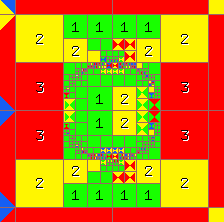
\includegraphics[width=0.25\textwidth]{mesh_irreg2.png}
\end{center}
\noindent
\vspace{-4mm}
\end{figure}
\noindent
{\em P. Solin, J. Cerveny, I. Dolezel: Arbitrary-Level Hanging Nodes and Automatic
Adaptivity in the hp-FEM, Math. Comput. Simul. 77 (2008), 117 - 132.}
\end{frame}


%Hanging nodes with DG
\begin{frame}
\frametitle{Arbitrary-level hanging nodes with DG}
\begin{center}
Element-wise assembling of the matrix \& rhs (jacobian \& residual)\\
Volume integrals ... \checkmark\\\ \\\ \\\ \\
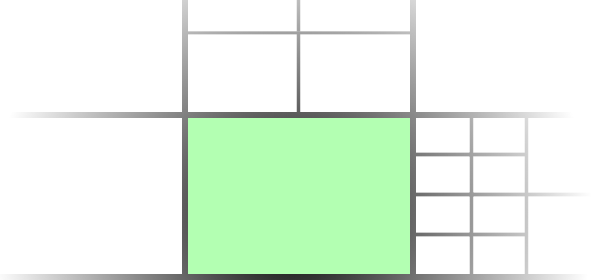
\includegraphics[width=0.7\textheight]{hndg/base.png}
\end{center}
\end{frame}
%Hanging nodes with DG
\begin{frame}
\frametitle{Arbitrary-level hanging nodes with DG}
\begin{center}
Surface integrals ... either boundary condition or numerical flux\\
Boundary condition representable as a numerical flux (with suitable boundary state)\\\ \\
Loop over the element edges: edge 1\\\ \\
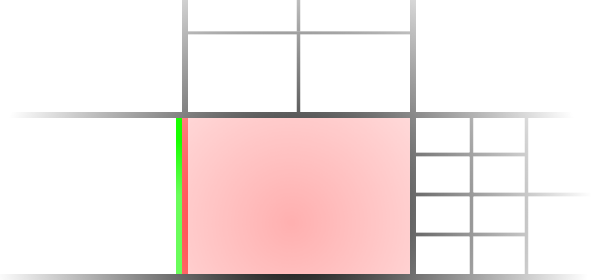
\includegraphics[width=0.7\textheight]{hndg/1.png}
\end{center}
\end{frame}
%Hanging nodes with DG
\begin{frame}
\frametitle{Arbitrary-level hanging nodes with DG}
\begin{center}
Surface integrals ... either boundary condition or numerical flux\\
Boundary condition representable as a numerical flux (with suitable boundary state)\\
Loop over the element edges: edge 2\\
We need to adjust the reference mapping(s) of the central element, so that the quadrature points coincide\\\ \\
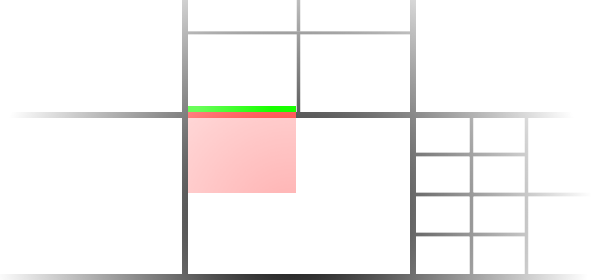
\includegraphics[width=0.7\textheight]{hndg/21.png}
\end{center}
\end{frame}
%Hanging nodes with DG
\begin{frame}
\frametitle{Arbitrary-level hanging nodes with DG}
\begin{center}
Surface integrals ... either boundary condition or numerical flux\\
Boundary condition representable as a numerical flux (with suitable boundary state)\\
Loop over the element edges: edge 2\\
We need to adjust the reference mapping(s) of the central element, so that the quadrature points coincide\\\ \\
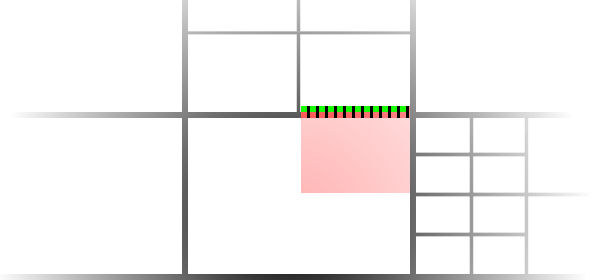
\includegraphics[width=0.7\textheight]{hndg/22.png}
\end{center}
\end{frame}
%Hanging nodes with DG
\begin{frame}
\frametitle{Arbitrary-level hanging nodes with DG}
\begin{center}
Surface integrals ... either boundary condition or numerical flux\\
Boundary condition representable as a numerical flux (with suitable boundary state)\\
Loop over the element edges: edge 3\\
We employ (almost) arbitrary level of hanging nodes.\\ \ \\
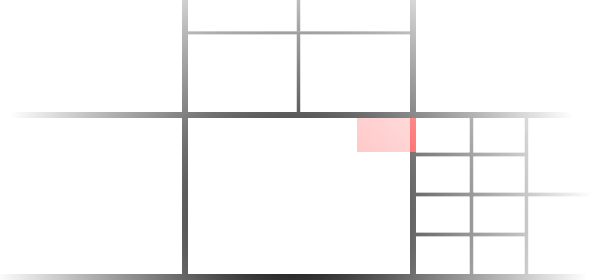
\includegraphics[width=0.7\textheight]{hndg/31.png}
\end{center}
\end{frame}
%Hanging nodes with DG
\begin{frame}
\frametitle{Arbitrary-level hanging nodes with DG}
\begin{center}
Surface integrals ... either boundary condition or numerical flux\\
Boundary condition representable as a numerical flux (with suitable boundary state)\\
Loop over the element edges: edge 3\\
We employ (almost) arbitrary level of hanging nodes.\\ \ \\
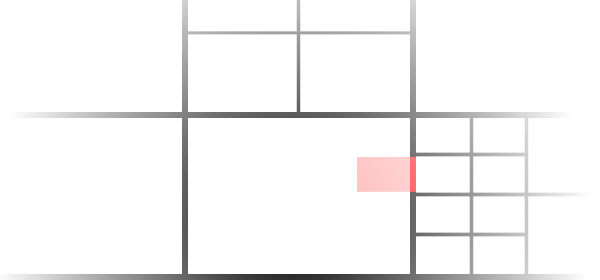
\includegraphics[width=0.7\textheight]{hndg/32.png}
\end{center}
\end{frame}
%Hanging nodes with DG
\begin{frame}
\frametitle{Arbitrary-level hanging nodes with DG}
\begin{center}
Surface integrals ... either boundary condition or numerical flux\\
Boundary condition representable as a numerical flux (with suitable boundary state)\\
Loop over the element edges: edge 3\\
We employ (almost) arbitrary level of hanging nodes.\\ \ \\
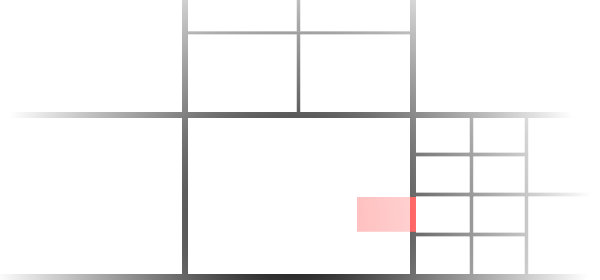
\includegraphics[width=0.7\textheight]{hndg/33.png}
\end{center}
\end{frame}
%Hanging nodes with DG
\begin{frame}
\frametitle{Arbitrary-level hanging nodes with DG}
\begin{center}
Surface integrals ... either boundary condition or numerical flux\\
Boundary condition representable as a numerical flux (with suitable boundary state)\\
Loop over the element edges: edge 3\\
We employ (almost) arbitrary level of hanging nodes.\\ \ \\
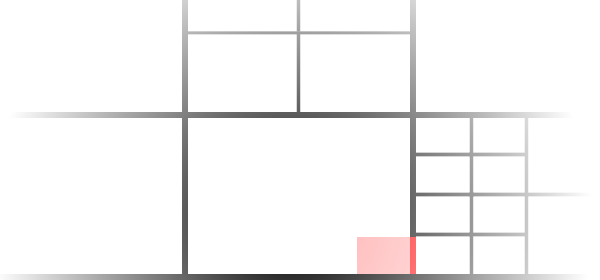
\includegraphics[width=0.7\textheight]{hndg/34.png}
\end{center}
\end{frame}
%Hanging nodes with DG
\begin{frame}
\frametitle{Arbitrary-level hanging nodes with DG}
\begin{center}
Surface integrals ... either boundary condition or numerical flux\\
Boundary condition representable as a numerical flux (with suitable boundary state)\\
An element may share an edge with a "bigger" element.\\ In this case we adjust the reference mapping of the NEIGHBOR element.\\ \ \\
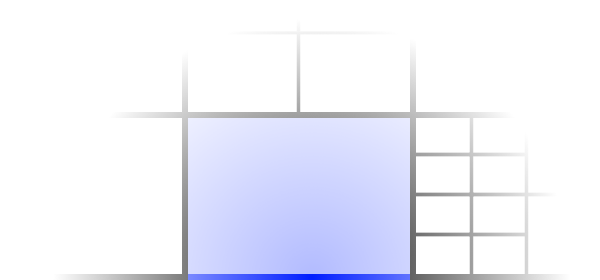
\includegraphics[width=0.7\textheight]{hndg/4.png}
\end{center}
\end{frame}

%Neighbor search
\begin{frame}
\frametitle{Search for neighbors in irregular mesh}
\begin{center}
How to find neighboring elements (one possible way)\\
\begin{itemize}
\item associative array (represented by a hash table) : ([vertex 1, vertex 2]) $\Rightarrow$ (shared edge)
\item associative array (represented by a hash table) : ([vertex 1, vertex 2]) $\Rightarrow$ (vertex in the middle)
\end{itemize}
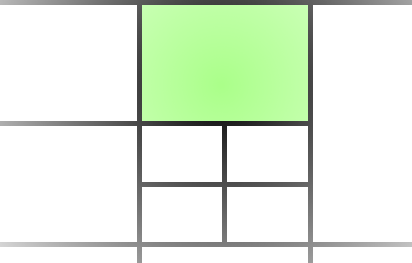
\includegraphics[width=0.7\textheight]{nsdg/base.png}
\end{center}
\end{frame}

\begin{frame}
\frametitle{Search for neighbors in irregular mesh}
\begin{center}
How to find neighboring elements (one possible way)\\
First edge - simple case\\ \ \\\ \\
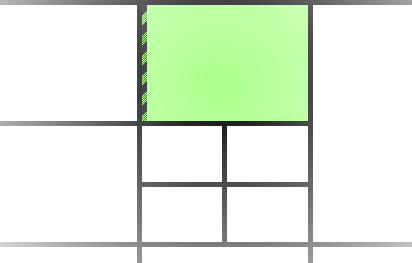
\includegraphics[width=0.7\textheight]{nsdg/10.png}
\end{center}
\end{frame}
\begin{frame}
\frametitle{Search for neighbors in irregular mesh}
\begin{center}
How to find neighboring elements (one possible way)\\
First edge - simple case\\
The edge structure (Edge) has pointers to 2 Elements if they share the level of refinement.\\\ \\
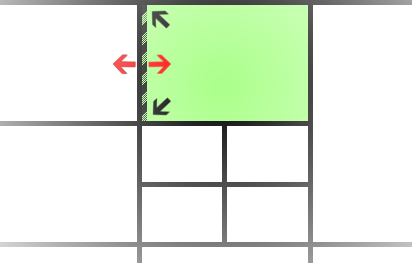
\includegraphics[width=0.7\textheight]{nsdg/11.png}
\end{center}
\end{frame}
\begin{frame}
\frametitle{Search for neighbors in irregular mesh}
\begin{center}
How to find neighboring elements (one possible way)\\
First edge - simple case\\
The correct Element is identified by id (we choose the correct one).\\\ \\
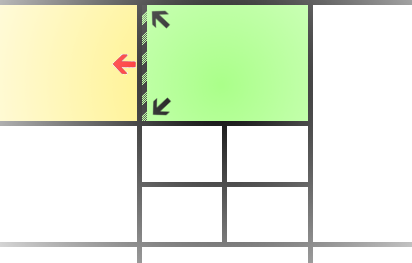
\includegraphics[width=0.7\textheight]{nsdg/12.png}
\end{center}
\end{frame}

\begin{frame}
\frametitle{Search for neighbors in irregular mesh}
\begin{center}
Second edge - multiple neighbors case\\
We use the array  ([vertex 1, vertex 2]) $\Rightarrow$ (vertex in the middle).\\
If we find a vertex, we repeat with [vertex 1, middle vertex], [middle vertex, vertex 2]\\
until we find an active edge between them.\\\ \\
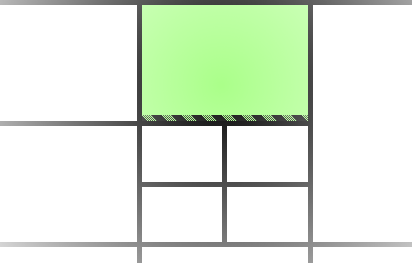
\includegraphics[width=0.7\textheight]{nsdg/20.png}
\end{center}
\end{frame}
\begin{frame}
\frametitle{Search for neighbors in irregular mesh}
\begin{center}
Second edge - multiple neighbors case\\
We use the array  ([vertex 1, vertex 2]) $\Rightarrow$ (vertex in the middle).\\
If we find a vertex, we repeat with [vertex 1, middle vertex], [middle vertex, vertex 2]\\
until we find an active edge between them.\\\ \\
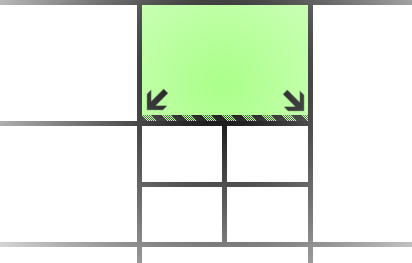
\includegraphics[width=0.7\textheight]{nsdg/21.png}
\end{center}
\end{frame}
\begin{frame}
\frametitle{Search for neighbors in irregular mesh}
\begin{center}
Second edge - multiple neighbors case\\
We use the array  ([vertex 1, vertex 2]) $\Rightarrow$ (vertex in the middle).\\
If we find a vertex, we repeat with [vertex 1, middle vertex], [middle vertex, vertex 2]\\
until we find an active edge between them.\\\ \\
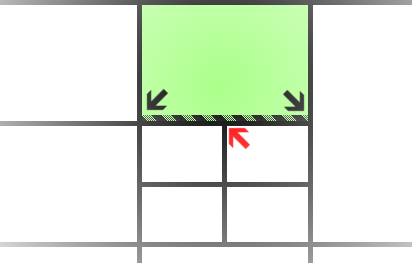
\includegraphics[width=0.7\textheight]{nsdg/22.png}
\end{center}
\end{frame}
\begin{frame}
\frametitle{Search for neighbors in irregular mesh}
\begin{center}
Second edge - multiple neighbors case\\
We use the array  ([vertex 1, vertex 2]) $\Rightarrow$ (vertex in the middle).\\
If we find a vertex, we repeat with [vertex 1, middle vertex], [middle vertex, vertex 2]\\
until we find an active edge between them.\\\ \\
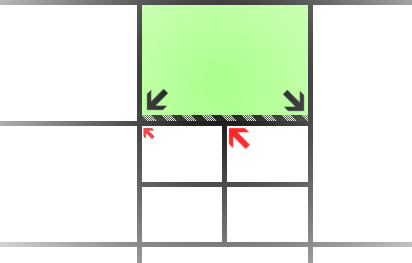
\includegraphics[width=0.7\textheight]{nsdg/23.png}
\end{center}
\end{frame}
\begin{frame}
\frametitle{Search for neighbors in irregular mesh}
\begin{center}
Second edge - multiple neighbors case\\
We use the array  ([vertex 1, vertex 2]) $\Rightarrow$ (vertex in the middle).\\
If we find a vertex, we repeat with [vertex 1, middle vertex], [middle vertex, vertex 2]\\
until we find an active edge between them.\\\ \\
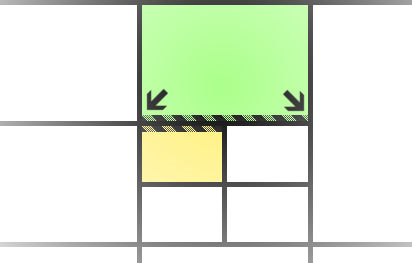
\includegraphics[width=0.7\textheight]{nsdg/24.png}
\end{center}
\end{frame}
\begin{frame}
\frametitle{Search for neighbors in irregular mesh}
\begin{center}
Second edge - multiple neighbors case\\
We use the array  ([vertex 1, vertex 2]) $\Rightarrow$ (vertex in the middle).\\
If we find a vertex, we repeat with [vertex 1, middle vertex], [middle vertex, vertex 2]\\
until we find an active edge between them.\\\ \\
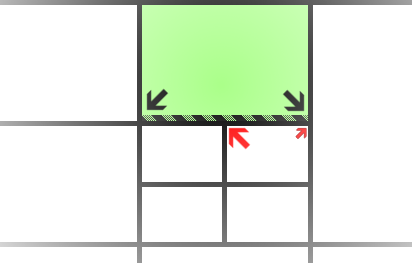
\includegraphics[width=0.7\textheight]{nsdg/25.png}
\end{center}
\end{frame}
\begin{frame}
\frametitle{Search for neighbors in irregular mesh}
\begin{center}
Second edge - multiple neighbors case\\
We use the array  ([vertex 1, vertex 2]) $\Rightarrow$ (vertex in the middle).\\
If we find a vertex, we repeat with [vertex 1, middle vertex], [middle vertex, vertex 2]\\
until we find an active edge between them.\\\ \\
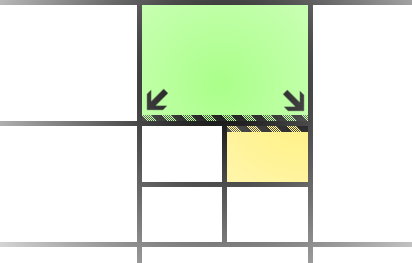
\includegraphics[width=0.7\textheight]{nsdg/26.png}
\end{center}
\end{frame}











\begin{frame}
\frametitle{Search for neighbors in irregular mesh}
\begin{center}
Third edge - neighbor element has to be adjusted for calculation\\
We have found neither a neighboring element, nor a vertex in the middle.\\
We use the hiearchic storage (a tree) of elements in the hp-mesh to get the parent Element.
Then we look for a neighbor of this "inactive" (not used for calculation) Element.\\\ \\
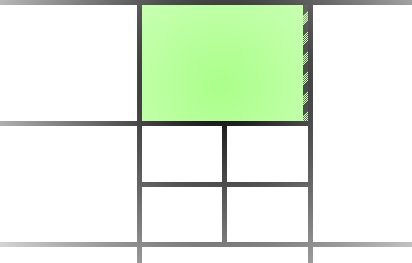
\includegraphics[width=0.7\textheight]{nsdg/30.png}
\end{center}
\end{frame}
\begin{frame}
\frametitle{Search for neighbors in irregular mesh}
\begin{center}
Third edge - neighbor element has to be adjusted for calculation\\
We have found neither a neighboring element, nor a vertex in the middle.\\
We use the hiearchic storage (a tree) of elements in the hp-mesh to get the parent Element.
Then we look for a neighbor of this "inactive" (not used for calculation) Element.\\\ \\
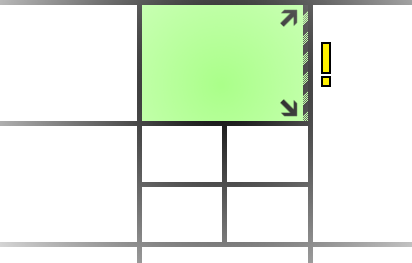
\includegraphics[width=0.7\textheight]{nsdg/31.png}
\end{center}
\end{frame}
\begin{frame}
\frametitle{Search for neighbors in irregular mesh}
\begin{center}
Third edge - neighbor element has to be adjusted for calculation\\
We have found neither a neighboring element, nor a vertex in the middle.\\
We use the hiearchic storage (a tree) of elements in the hp-mesh to get the parent Element.
Then we look for a neighbor of this "inactive" (not used for calculation) Element.\\\ \\
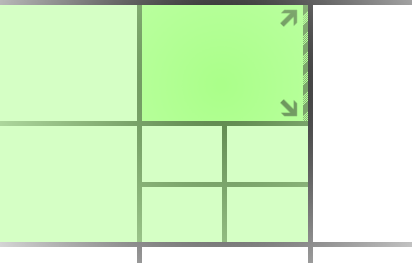
\includegraphics[width=0.7\textheight]{nsdg/32.png}
\end{center}
\end{frame}
\begin{frame}
\frametitle{Search for neighbors in irregular mesh}
\begin{center}
Third edge - neighbor element has to be adjusted for calculation\\
We have found neither a neighboring element, nor a vertex in the middle.\\
We use the hiearchic storage (a tree) of elements in the hp-mesh to get the parent Element.
Then we look for a neighbor of this "inactive" (not used for calculation) Element.\\\ \\
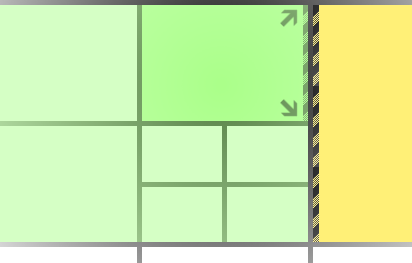
\includegraphics[width=0.7\textheight]{nsdg/33.png}
\end{center}
\end{frame}




\def\Tiny{\fontsize{6pt}{0pt}\selectfont}
\def\Tinya{\fontsize{8pt}{0pt}\selectfont}
\def\Tinyb{\fontsize{7pt}{0pt}\selectfont}
\definecolor{mygreen}{rgb}{0.23,0.738,0}
\begin{frame}[fragile]
\frametitle{Hermes parallel hp-FEM \& hp-DG (multimesh) assembling of (nonlinear) problems}
\begin{Verbatim}[commandchars=\\\{\}, fontsize=\Tiny]
 1 \textcolor{blue}{#pragma omp parallel} shared(traverse_master, matrix, right_hand_side)
 2 num_threads(Hermes2DApi.getParamValue(Hermes::Hermes2D::numThreads))
 3 \{
 4 \textcolor{blue}{#pragma} omp for schedule(dynamic, CHUNKSIZE)
 5   \textcolor{blue}{for} (state_i = 0\textcolor{blue}{;} state_i < num_states\textcolor{blue}{;} state_i++)
 6   \{
 7 \textcolor{blue}{#pragma omp critical} (get_next_state)
 8     current_state = traverse[thread_id].get_next_state
           (&traverse_master.top, &traverse_master.id)\textcolor{blue}{;}
 9
10     basis_functions = basis_functions[thread_id]\textcolor{blue}{;}
11     test_functions = test_functions[thread_id]\textcolor{blue}{;}
12     ref_mappings = refmaps[thread_id]\textcolor{blue}{;}
13     assembly_lists = assembly_lists[thread_id]\textcolor{blue}{;}
14     forms = &(forms[thread_id].front())\textcolor{blue}{;}
15 
16     \textcolor{mygreen}{// Assemble volumetric forms and surface forms corresponding to boundary conditions.}
17     assemble_one_state(basis_functions, test_functions, ref_mappings, assembly_lists,
         &current_state, forms)\textcolor{blue}{;}
18 
19     \textcolor{mygreen}{// DG}
20     \textcolor{blue}{for} (edge = 0\textcolor{blue}{;} edge < current_state.get_number_of_edges()\textcolor{blue}{;} edge++)
21     \{
22       \textcolor{mygreen}{// Find the neighbors of this element over this edge.}
23       neighbor_groups[edge]->find_neighbors(&current_state, edge, basis_functions, 
           test_functions, ref_mappings, assembly_lists, forms)\textcolor{blue}{;}
24       
25       \textcolor{mygreen}{// Go through possibly many neighbors and assemble the forms.}
26       \textcolor{blue}{for} (neighbor = 0\textcolor{blue}{;} neighbor < neighbor_groups[edge].number_of_neighbors\textcolor{blue}{;} neighbor++)
27         neighbor_groups[edge]->assemble_one_DG_edge(neighbor)\textcolor{blue}{;}
28     \}
29   \}
30 \}
\end{Verbatim}
\end{frame}
\begin{frame}[fragile]
\frametitle{Hermes parallel hp-FEM \& hp-DG (multimesh) assembling of (nonlinear) problems}
\begin{Verbatim}[commandchars=\\\{\}, fontsize=\Tiny]
 1\Tinya \textcolor{blue}{#pragma omp parallel} shared(traverse_master, matrix, right_hand_side)
 2\Tinya num_threads(Hermes2DApi.getParamValue(Hermes::Hermes2D::numThreads))
 3 \{
 4 \textcolor{blue}{#pragma} omp for schedule(dynamic, CHUNKSIZE)
 5   \textcolor{blue}{for} (state_i = 0\textcolor{blue}{;} state_i < num_states\textcolor{blue}{;} state_i++)
 6   \{
 7 \textcolor{blue}{#pragma omp critical} (get_next_state)
 8     current_state = traverse[thread_id].get_next_state
           (&traverse_master.top, &traverse_master.id)\textcolor{blue}{;}
 9
10     basis_functions = basis_functions[thread_id]\textcolor{blue}{;}
11     test_functions = test_functions[thread_id]\textcolor{blue}{;}
12     ref_mappings = refmaps[thread_id]\textcolor{blue}{;}
13     assembly_lists = assembly_lists[thread_id]\textcolor{blue}{;}
14     forms = &(forms[thread_id].front())\textcolor{blue}{;}
15 
16     \textcolor{mygreen}{// Assemble volumetric forms and surface forms corresponding to boundary conditions.}
17     assemble_one_state(basis_functions, test_functions, ref_mappings, assembly_lists,
         &current_state, forms)\textcolor{blue}{;}
18 
19     \textcolor{mygreen}{// DG}
20     \textcolor{blue}{for} (edge = 0\textcolor{blue}{;} edge < current_state.get_number_of_edges()\textcolor{blue}{;} edge++)
21     \{
22       \textcolor{mygreen}{// Find the neighbors of this element over this edge.}
23       neighbor_groups[edge]->find_neighbors(&current_state, edge, basis_functions, 
           test_functions, ref_mappings, assembly_lists, forms)\textcolor{blue}{;}
24       
25       \textcolor{mygreen}{// Go through possibly many neighbors and assemble the forms.}
26       \textcolor{blue}{for} (neighbor = 0\textcolor{blue}{;} neighbor < neighbor_groups[edge].number_of_neighbors\textcolor{blue}{;} neighbor++)
27         neighbor_groups[edge]->assemble_one_DG_edge(neighbor)\textcolor{blue}{;}
28     \}
29   \}
30 \}
\end{Verbatim}
\end{frame}
\begin{frame}[fragile]
\frametitle{Hermes parallel hp-FEM \& hp-DG (multimesh) assembling of (nonlinear) problems}
\begin{Verbatim}[commandchars=\\\{\}, fontsize=\Tiny]
 1 \textcolor{blue}{#pragma omp parallel} shared(traverse_master, matrix, right_hand_side)
 2 num_threads(Hermes2DApi.getParamValue(Hermes::Hermes2D::numThreads))
 3 \{
 4 \Tinya\textcolor{blue}{#pragma} omp for schedule(dynamic, CHUNKSIZE)
 5   \Tinya\textcolor{blue}{for} (state_i = 0\textcolor{blue}{;} state_i < num_states\textcolor{blue}{;} state_i++)
 6   \{
 7 \Tinya\textcolor{blue}{#pragma omp critical} (get_next_state)
 8    \Tinya current_state = traverse[thread_id].get_next_state
           \Tinya(&traverse_master.top, &traverse_master.id)\textcolor{blue}{;}
 9
10     basis_functions = basis_functions[thread_id]\textcolor{blue}{;}
11     test_functions = test_functions[thread_id]\textcolor{blue}{;}
12     ref_mappings = refmaps[thread_id]\textcolor{blue}{;}
13     assembly_lists = assembly_lists[thread_id]\textcolor{blue}{;}
14     forms = &(forms[thread_id].front())\textcolor{blue}{;}
15 
16     \textcolor{mygreen}{// Assemble volumetric forms and surface forms corresponding to boundary conditions.}
17     assemble_one_state(basis_functions, test_functions, ref_mappings, assembly_lists,
         &current_state, forms)\textcolor{blue}{;}
18 
19     \textcolor{mygreen}{// DG}
20     \textcolor{blue}{for} (edge = 0\textcolor{blue}{;} edge < current_state.get_number_of_edges()\textcolor{blue}{;} edge++)
21     \{
22       \textcolor{mygreen}{// Find the neighbors of this element over this edge.}
23       neighbor_groups[edge]->find_neighbors(&current_state, edge, basis_functions, 
           test_functions, ref_mappings, assembly_lists, forms)\textcolor{blue}{;}
24       
25       \textcolor{mygreen}{// Go through possibly many neighbors and assemble the forms.}
26       \textcolor{blue}{for} (neighbor = 0\textcolor{blue}{;} neighbor < neighbor_groups[edge].number_of_neighbors\textcolor{blue}{;} neighbor++)
27         neighbor_groups[edge]->assemble_one_DG_edge(neighbor)\textcolor{blue}{;}
28     \}
29   \}
30 \}
\end{Verbatim}
\end{frame}
\begin{frame}[fragile]
\frametitle{Hermes parallel hp-FEM \& hp-DG (multimesh) assembling of (nonlinear) problems}
\begin{Verbatim}[commandchars=\\\{\}, fontsize=\Tiny]
 1 \textcolor{blue}{#pragma omp parallel} shared(traverse_master, matrix, right_hand_side)
 2 num_threads(Hermes2DApi.getParamValue(Hermes::Hermes2D::numThreads))
 3 \{
 4 \textcolor{blue}{#pragma} omp for schedule(dynamic, CHUNKSIZE)
 5   \textcolor{blue}{for} (state_i = 0\textcolor{blue}{;} state_i < num_states\textcolor{blue}{;} state_i++)
 6   \{
 7 \textcolor{blue}{#pragma omp critical} (get_next_state)
 8     current_state = traverse[thread_id].get_next_state
           (&traverse_master.top, &traverse_master.id)\textcolor{blue}{;}
 9
10    \Tinya basis_functions = basis_functions[thread_id]\textcolor{blue}{;}
11    \Tinya test_functions = test_functions[thread_id]\textcolor{blue}{;}
12    \Tinya ref_mappings = refmaps[thread_id]\textcolor{blue}{;}
13    \Tinya assembly_lists = assembly_lists[thread_id]\textcolor{blue}{;}
14    \Tinya forms = &(forms[thread_id].front())\textcolor{blue}{;}
15 
16     \textcolor{mygreen}{// Assemble volumetric forms and surface forms corresponding to boundary conditions.}
17     assemble_one_state(basis_functions, test_functions, ref_mappings, assembly_lists,
         &current_state, forms)\textcolor{blue}{;}
18 
19     \textcolor{mygreen}{// DG}
20     \textcolor{blue}{for} (edge = 0\textcolor{blue}{;} edge < current_state.get_number_of_edges()\textcolor{blue}{;} edge++)
21     \{
22       \textcolor{mygreen}{// Find the neighbors of this element over this edge.}
23       neighbor_groups[edge]->find_neighbors(&current_state, edge, basis_functions, 
           test_functions, ref_mappings, assembly_lists, forms)\textcolor{blue}{;}
24       
25       \textcolor{mygreen}{// Go through possibly many neighbors and assemble the forms.}
26       \textcolor{blue}{for} (neighbor = 0\textcolor{blue}{;} neighbor < neighbor_groups[edge].number_of_neighbors\textcolor{blue}{;} neighbor++)
27         neighbor_groups[edge]->assemble_one_DG_edge(neighbor)\textcolor{blue}{;}
28     \}
29   \}
30 \}
\end{Verbatim}
\end{frame}
\begin{frame}[fragile]
\frametitle{Hermes parallel hp-FEM \& hp-DG (multimesh) assembling of (nonlinear) problems}
\begin{Verbatim}[commandchars=\\\{\}, fontsize=\Tiny]
 1 \textcolor{blue}{#pragma omp parallel} shared(traverse_master, matrix, right_hand_side)
 2 num_threads(Hermes2DApi.getParamValue(Hermes::Hermes2D::numThreads))
 3 \{
 4 \textcolor{blue}{#pragma} omp for schedule(dynamic, CHUNKSIZE)
 5   \textcolor{blue}{for} (state_i = 0\textcolor{blue}{;} state_i < num_states\textcolor{blue}{;} state_i++)
 6   \{
 7 \textcolor{blue}{#pragma omp critical} (get_next_state)
 8     current_state = traverse[thread_id].get_next_state
           (&traverse_master.top, &traverse_master.id)\textcolor{blue}{;}
 9
10     basis_functions = basis_functions[thread_id]\textcolor{blue}{;}
11     test_functions = test_functions[thread_id]\textcolor{blue}{;}
12     ref_mappings = refmaps[thread_id]\textcolor{blue}{;}
13     assembly_lists = assembly_lists[thread_id]\textcolor{blue}{;}
14     forms = &(forms[thread_id].front())\textcolor{blue}{;}
15 
16     \textcolor{mygreen}{// Assemble volumetric forms and surface forms corresponding to boundary conditions.}
17     assemble_one_state(basis_functions, test_functions, ref_mappings, assembly_lists,
         &current_state, forms)\textcolor{blue}{;}
18 
19     \Tinya\textcolor{mygreen}{// DG}
20     \Tinya\textcolor{blue}{for} (edge = 0\textcolor{blue}{;} edge < current_state.get_number_of_edges()\textcolor{blue}{;} edge++)
21     \Tinyb\{
22       \Tinyb\textcolor{mygreen}{// Find the neighbors of this element over this edge.}
23       neighbor_groups[edge]->find_neighbors(&current_state, edge, basis_functions, 
          \Tinyb test_functions, ref_mappings, assembly_lists, forms)\textcolor{blue}{;}
24       
25       \Tinyb\textcolor{mygreen}{// Go through possibly many neighbors and assemble the forms.}
26       \textcolor{blue}{for} (neighbor = 0\textcolor{blue}{;} neighbor < neighbor_groups[edge].number_of_neighbors\textcolor{blue}{;} neighbor++)
27        \Tinyb neighbor_groups[edge]->assemble_one_DG_edge(neighbor)\textcolor{blue}{;}
28     \Tinyb\}
29   \}
30 \}
\end{Verbatim}
\end{frame}


%Adaptive mechanism
\begin{frame}
\frametitle{Adaptive algorithm - error estimator based on reference and coarse solutions}
\begin{center}
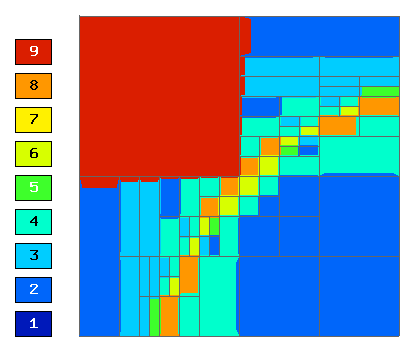
\includegraphics[width=0.45\textheight]{refsln/screen002.png}
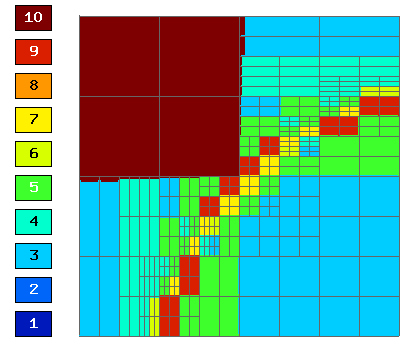
\includegraphics[width=0.45\textheight]{refsln/screen003.png}
\end{center}
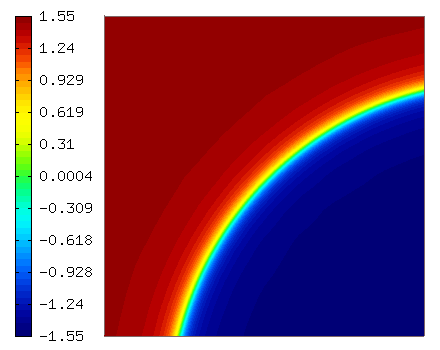
\includegraphics[width=0.6\textheight]{refsln/screen001.png}
\end{frame}













%Discretization
\begin{frame}
\frametitle{Discretization of time dependent problems}
\begin{itemize}
\item Rothe's method\ \\
\begin{itemize}
\item discretization in time first
\item discretized problem at each time level solved by adaptive hp-FEM
\end{itemize}
\item dynamical meshes
\begin{itemize}
\item meshes evolve in time
\item independent of each other
\\
\includegraphics[width=0.5\textheight]{shot0001.png}
\end{itemize}
\end{itemize}
\end{frame}
\begin{frame}
\frametitle{Discretization of time dependent problems}
\begin{itemize}
\item Rothe's method\ \\
\begin{itemize}
\item discretization in time first
% system of ODEs
\item discretized problem at each time level solved by adaptive hp-FEM
\end{itemize}
\item dynamical meshes
\begin{itemize}
\item meshes evolve in time
\item independent of each other
\\
\includegraphics[width=0.5\textheight]{shot0002.png}
\end{itemize}
\end{itemize}
\end{frame}
\begin{frame}
\frametitle{Discretization of time dependent problems}
\begin{itemize}
\item Rothe's method\ \\
\begin{itemize}
\item discretization in time first
% system of ODEs
\item discretized problem at each time level solved by adaptive hp-FEM
\end{itemize}
\item dynamical meshes
\begin{itemize}
\item meshes evolve in time
\item independent of each other
\\
\includegraphics[width=0.5\textheight]{shot0003.png}
\end{itemize}
\end{itemize}
\end{frame}
\begin{frame}
\frametitle{Discretization of time dependent problems}
\begin{itemize}
\item Rothe's method\ \\
\begin{itemize}
\item discretization in time first
% system of ODEs
\item discretized problem at each time level solved by adaptive hp-FEM
\end{itemize}
\item dynamical meshes
\begin{itemize}
\item meshes evolve in time
\item independent of each other
\\
\includegraphics[width=0.5\textheight]{shot0004.png}
\end{itemize}
\end{itemize}
\end{frame}
\begin{frame}
\frametitle{Discretization of time dependent problems}
\begin{itemize}
\item Rothe's	 method\ \\
\begin{itemize}
\item discretization in time first
% system of ODEs
\item discretized problem at each time level solved by adaptive hp-FEM
\end{itemize}
\item dynamical meshes
\begin{itemize}
\item meshes evolve in time
\item independent of each other
\\
\includegraphics[width=0.5\textheight]{shot0005.png}
\end{itemize}
\end{itemize}
\end{frame}

%Time discretization
\begin{frame}
\frametitle{Discretization in time}
Semi-implicit discretization\ \\
\begin{itemize}
\item linear terms discretized implicitly
\item nonlinear terms explicitly
\item possible increase of time step % with preserved stability
\end{itemize}
\end{frame}

%Space discretization
\begin{frame}
\frametitle{Discretization in space}
\begin{itemize}
\item
adaptive hp-DG for the Euler equations
\begin{itemize}
\item Steger-Warming numerical flux (easy linearization) %makes it possible to carry out the 
\item	
polynomial orders up to 10 (orders used in practice are lower)
\item
Shock capturing
\item
Flux limiting
\end{itemize}
\item
adaptive hp-FEM for the advection-diffusion equation
\begin{itemize}
\item
polynomial orders up to 10
\end{itemize}
\end{itemize}
\end{frame}



\begin{frame}
\frametitle{Outlook}
\begin{center}
\begin{itemize}
\item - Use the fully implicit scheme
\item - Use JFNK method (NOX package from the Trilinos library)
\item - Use the "full" Newton's method
\end{itemize}
\end{center}
\end{frame}


\begin{frame}
\frametitle{Comparison of meshes}
\begin{center}
\Large
Thank you for your attention.
\end{center}
\end{frame}

\end{document}
